\section{FE-MSM}
\label{sec:fe-msm}
FE-MSM consists of two stages: (i) a treatment model that 
estimates the propensity scores, conditioning on both observed 
covariates and individual fixed effects that capture the 
unmeasured time-invariant confounding, 
and (ii) a marginal structural model that uses the 
estimated propensity scores in stage one to adjust for 
confounding using IPTW. FE-MSM can be seen as a very direct way of 
bringing back the sequential 
ignorability assumption where we suspect of unmeasured time-invariant 
confounding. More formally, the identification of 
the causal effect of interest relies on the following assumption:
\begin{idassumpFE}[Unit-specific ignorability]\label{ass:FE-unit-specific-ignor}
    Let $\alpha_i$ be a time-invariant unmeasured unidimensional random variable, For 
    all $i$, $t$ and $\bar{a}_t$,
    \[
    \{ Y_{i}(\bar{a}_{T}),\, \underbar{X}_{i,t+1}(\bar a_t) \}
\;\perp\!\!\!\perp\;
A_{it}
\;\big|\;
\bar{X}_{it},\,
\bar A_{i,t-1} = \bar a_{t-1},\,
\alpha_i. \]

\end{idassumpFE}

Assumption \ref{ass:FE-unit-specific-ignor} states that conditioned on 
the past treatment and covariate history, as well as 
the unmeasured fixed effect $\alpha_i$, 
the treatment assignment at time $t$ is independent of the future 
potential outcomes and covariates. Under this assumption, the truncated potential 
outcome $\mathbb{E}[Y_i(\underline{a}_{T-k})]$ can be nonparametrically identified as follows

\begin{equation}
    \mathbb{E}\bigl[Y_i(\underbar{a}_{T-k})\bigr]
    =
    \mathbb{E}\left[
    \frac{\mathbf{1}\bigl(\underbar{A}_{i,T-k} = \underbar{a}_{T-k}\bigr)\, Y_i}
    {\prod_{t=T-k}^{T} \pi_{it}^{a_t} (1 - \pi_{it})^{1 - a_t}}
    \right].
\end{equation}
Where $\pi_{it} = \Pr(A_{it} = 1 \mid \bar X_{it}, \bar A_{i,t-1}, \alpha_i)$. 

In practice, this probability is being estimated from the data using a parametric model. This model 
requires to be correctly specified up to the unit-specific fixed effect for IPTW to be consistant.

\begin{modassumpFE}[Correct specification of the propensity score model up to time-invariant unmeasured heterogeneity]
\label{ass:FE-ps-correct}
The parametric model
There exists an \emph{unmeasured}, unit-specific, time-constant variable $\alpha_i$ capturing
time-invariant unmeasured heterogeneity in treatment assignment, and a known model class
$\{\pi_{it}(\cdot;\theta,z)\}_{\theta\in\Theta}$ (parametric in $\theta$), such that for all individuals $i$
and times $t$,
\[
\mathbb{P}\!\bigl(D_{it}=1 \,\big|\, \bar X_{it},\, \bar A_{i,t-1},\, \alpha_i \bigr)
=
\pi_{it}\!\left(\bar X_{it},\, \bar A_{i,t-1};\, \theta_0,\, \alpha_i\right),
\]
for some finite-dimensional parameter vector $\theta_0$. In other words, the functional form
in $\theta$ is correctly specified \emph{conditional on} $\alpha_i$ (i.e., the model is correct \emph{up to}
the unmeasured heterogeneity $\alpha_i$).
\end{modassumpFE}

\begin{idassumpFE}[Positivity assumption]
    
    
\end{idassumpFE}
\begin{figure}
    \centering
    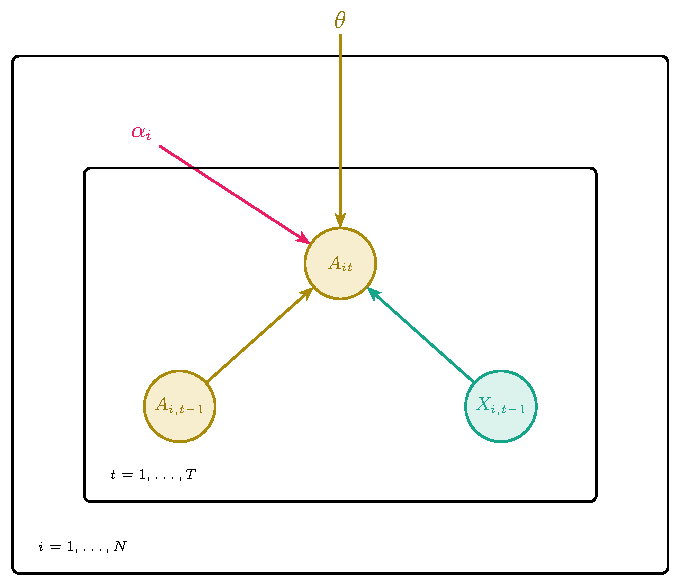
\includegraphics[width=0.8\linewidth]{figures/build/fixed_effect_dag.pdf}
    \caption{
    Plate diagram of the the conditional assignment likelihood
    for the fixed-effects propensity-score model. The likelihood factorizes as
    $
    p(\mathbf{A} \mid \mathbf{X}, \mathbf{Z}, \theta)
    =
    \prod_{i,t}
    p\!\left(A_{it} \mid A_{i,t-1}, X_{i,t-1}, Z_i, \theta\right).
    $
    We do not specify a model for the 
    joint distribution of $(\mathbf{X}, \mathbf{Z})$. Note that, 
    since $\alpha_i$ is considered as a parameter and not a random variable 
    in this method, 
    it does not have a node around it.
    }
\label{fig:fixed_effect_architecture}
\end{figure}
